\documentclass[10pt,a4paper]{article}
%\usepackage[utf8]{inputenc}<--- no more needed in up-to-date distribution
\usepackage[T1]{fontenc}
\usepackage{threeparttable}
\usepackage{tikz}
\usetikzlibrary{matrix}

\begin{document}
    \begin{table}\centering
     \begin{threeparttable} 
        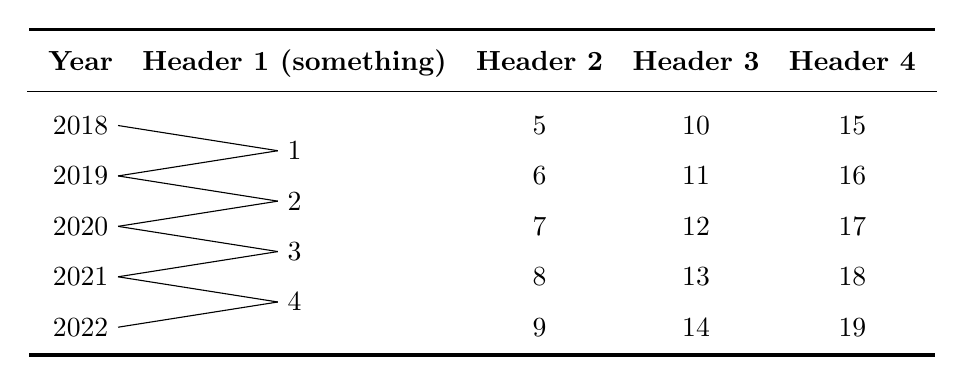
\begin{tikzpicture} 
            \matrix[matrix of nodes, 
                row sep=-4pt, 
                column sep=4pt, 
                row 1/.style={font=\bfseries, text height=8pt, text depth=4pt}] (mymatr)
            {  
            Year & Header 1 (something) &  Header 2 & Header 3 & Header 4 \\[10pt]
            2018 &  & 5 & 10 & 15 \\
            & 1 \\
            2019 &  & 6 & 11 & 16 \\
            & 2 \\
            2020 & & 7 & 12 & 17 \\
            & 3 \\
            2021 & & 8 & 13 & 18 \\
            & 4 \\
            2022 & & 9 & 14 & 19 \\
            };
            \foreach \ind
               [evaluate=\ind as \indpre using int(\ind-1),
               evaluate=\ind as \indpost using int(\ind+1)
               ] in {3, 5, 7, 9} 
               { 
               \draw (mymatr-\indpre-1.east) --
               (mymatr-\ind-2.west);
              \draw (mymatr-\indpost-1.east) --
               (mymatr-\ind-2.west);
               }
            % hlines
            \draw[very thick] (mymatr.north west) -- (mymatr.north east); 
            \draw[shorten >=-4pt, shorten <=-4pt] (mymatr-1-1.south west) -- (mymatr-1-5.south east); 
            \draw[very thick] (mymatr.south west) -- (mymatr.south east); 
        \end{tikzpicture} 
        \begin{tablenotes}[para]\small
            Note: I added the headers only to show how to manage them with a Ti\emph{k}Zmatrix.
        \end{tablenotes}
        \end{threeparttable}    
    \end{table}
\end{document}